\subsection{GPU ISA Encoding Solver and Assembler}
We need the GPU ISA encoding information to build a GPU assembler.
However, GPU vendors do not release this information as CPU vendors.
Previous third-party work to build GPU assemblers~\cite{decuda,asfermi,maxas} also
involves cracking GPU ISA encodings, whereas no cracking process is explicitly reported.
Our solver is proposed to make cracking GPU ISA encodings easy, automatic and portable to future GPUs.
%We do not know whether their methods is able to crack ISA encodings of next generation GPU.


Operands could be registers (e.g. {\tt R5}), 
global memory (e.g. {\tt [R6+0x20]}), constant memory (e.g. {\tt C[0x2][0x40]}), shared memory (e.g. {\tt [0x50]}), immediate values (e.g. {\tt 0x9} and {\tt1.5}), or predicate registers (e.g. {\tt P3})~\cite{ptx2015isa}.
We observe that an operand name always includes a number, thus the encoding of an operand can be inferred by its name.
For example, the register operand {\tt R5} is inferred from $101$ in binary format, while the immediate value {\tt 0x9} is $1001$. 
%Besides, the fixed lengths of these fields allow us to determine their positions \jled{and lengths, don't need to specify lengths here.} relatively easily and hence to encode them. 
The encodings of opcodes and modifiers are mnemonic symbols which can not be expressed as binary literally, thus they must be enumerated in their encoding space.
We design a heuristic algorithm on a pruned search space to determine the positions of opcodes and modifiers.
Modifiers are instruction-sensitive which means modifiers in the same type may have different encodings for different instructions. 
As an example, masks of type-size modifier for instructions {\tt LD} and {\tt LDG} are in different binary positions. 
Hence, every instruction's modifier need to be processed independently. 

We write a simple generator to produce PTX instructions with various modifiers as the samples in figure~\ref{fig:workflow}.
These PTX files are compiled to cubin files by {\tt ptxas}, and then disassembled by {\tt cuobjdump} to generate their native assemblies. 
Figure~\ref{fig:imm} shows a native assembly instruction example consisting of {\tt opcode}, {\tt operand}, and {\tt modifier} fields.
We express a native assembly instruction in a struct variable $instMap$\jli{$inst$}, which is the input of our solver.
%In this way, we generate real assembly instruction and their 64-bit encoding, which is the input of solver algorithm.
%We disassmble libcublas.so to generate instruction and their corresponing 64-bit encodings. There are $1537123$ different encodings of cublas 7.0 library in total.
\begin{figure}[htbp]
\begin{center}
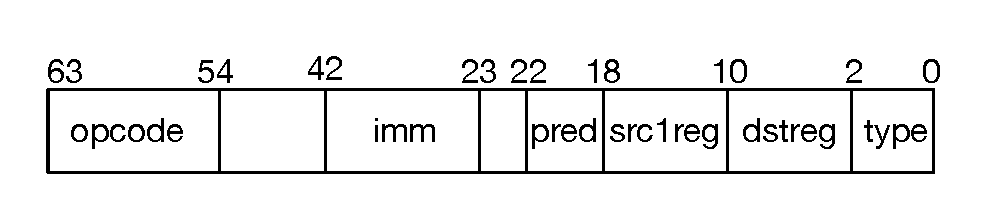
\includegraphics[scale=0.5]{imm}
    \caption{\jli{delete ``Immediate position in ''}{\tt IADD} instruction}
\label{fig:imm}
\end{center}
\end{figure}

\jli{Add explanation for the three algorithms in each subsection.}

\subsubsection{Opcode Encoding Solver}
Unlike operands, opcodes and modifiers do not show their encodings literally. One possible way to crack the operand 
encodings is to write intermediate codes
based on NVIDIA PTX syntax, and generate encoding by NVIDIA toolchain.
Subsequently, the opcodes can be achieved by stripping out operand masks, and
flags can be found by stripping out both opcodes and operand masks.
However, the uncompleteness of NVIDIA document hinders us from finding out all the opcodes and instruction modifiers. 
Another feasible way is to find the bit positions which represents opcode, then
enumerate all the possible binary combinations after stripping out operand masks as Algorithm~\ref{algo:opcode} shows.
By running Algorithm~\ref{algo:opcode}, we find that both the top $10$ bits and lower $2$ bits represent opcode on Kepler GPU.
Thus, we only enumerate these opcode bits which generate an acceptable search space. Finally, we find 
the minimal opcode without any flags. The time complexity is O(N*64), where N
is disassembly input generated by PTX, $64$ represents probing flipping 64
bits.

\begin{algorithm}[htbp]
      \caption{Opcode Solver}\label{algo:opcode}
  \begin{algorithmic}[1]
      \State \textbf {Input:} part diassembly generated by PTX
      \State \textbf {Onput:} Opcodes' positions in 64-bit encoding
      \For {$i \gets 0, N$}
	  %\LineComment {fetch an instruction from generated database \jled{what's the database?}}
      %\State \For i in instMap
      \LineComment {structure of inst\{ op, enc64, oprdType, oprd\}}
      \State inst = instParser(line[i])
      %\State $inst \gets instMap[i]$
      \State $enc \gets inst.enc64$
	  \LineComment {check each bit of $enc$ for opcode}
      \For {$j \gets 0, 63$}
      %\LineComment {if bit $j$ not operand bit and its value is 0} % \jled{what about enc[j]!=0? No need to check if it is opcode?}}
      %\If {notOprd($enc[j]$) and $enc[j] = 0$}
      \LineComment {flip bit $j$}
      \State nEnc = xor($enc, 1<<j$)
	  \LineComment {disassemble new encoding nEnc}
      \State nInst=nvdisasm(nEnc)
	  \LineComment {bit $j$ belongs to an opcode if it is changed }
      \If { isvalid(nInst) and $nInst.op\neq inst.op$}
      \State put($j$, $opBits$)
      %\EndIf
      \EndIf
      \EndFor
      \EndFor
      \State \textbf{Return} opBits %\jled{All instructions' opcodes are stored in opBits?}
  \end{algorithmic}
\end{algorithm}

\subsubsection{Operand Position Solver}
Each opcode may have different numbers and types of operands, we had better probe operand positions by both opcode and operand type. 
For example, {\tt FADD} has three kinds of operand types: {\tt FADD} R1,R2,R3; {\tt FADD} R1, R2,
C[0x0][0x40]; {\tt FADD} R1, R2, 0.5;. We represent the operand type as a string:
RRR, RRC, RRI for {\tt FADD} instruction, where R, C and I denotes register, constant
memory and immediate respectively. Then we probe bit position for each type.
The main idea is shown in Algorithm~\ref{algo:operand}.
\begin{algorithm}[htbp]
      \caption{Operand Solver}\label{algo:operand}
  \begin{algorithmic}[1]
      \State \textbf {Input:} diassembly with all the opcodes generated by opcode solver
      \State \textbf {Onput:} Operand positions for each opcode
      \LineComment {A hash table to check if the operand bit position of an opcode with operandType is probed}
      \State {visited=\{\}}
      \For {$i \gets 0, N$}
	  %\LineComment {fetch an instruction from generated database \jled{what's the database?}}
      \LineComment {structure of inst\{ op, enc64, oprdType, oprd\}}
      \State inst = instParser(line[i])
      %\State $inst \gets instMap[i]$
      %\State $enc \gets inst.enc64$
	  \LineComment {check each bit of $enc$ for opcode}
      \For {$j \gets 0, 63$}
      %\LineComment {if bit $j$ not operand bit and its value is 0} % \jled{what about enc[j]!=0? No need to check if it is opcode?}}
      %\If {notOprd($enc[j]$) and $enc[j] = 0$}
      \LineComment {flip bit $j$}
      \State nEnc = xor($enc, j$)
	  \LineComment {disassemble new encoding nEnc}
      \State nInst=nvdisasm(nEnc)
	  \LineComment {bit $j$ belongs to an operand }
      \If {ith = whichChange(origin,new) > 0}
      \State pos[origin.op][origin.oprdType][ith].append(j)
      \State visited[origin.op][origin.oprdType] = 1
      %\State put($j$, $operandBits$)
      %\EndIf
      \EndIf
      \EndFor
      \EndFor
      \State \textbf{Return} pos %\jled{All instructions' opcodes are stored in opBits?}
  \end{algorithmic}
\end{algorithm}
%Algorithm~\ref{algo:int_solver} shows the pseudocode for immediate operand decoding process. 
%The basic idea is matching the binary encoding of an operand in $64$-bit instruction encoding and finding
%position until the position is unique. The input instructions are from disassembly codes.
%First, we randomly pick up an instruction that has the field we want to probe and represent the field in binary by its 
%name. Second, we match the operand binary in $64$-bit instruction encoding and find possible positions. Third, we 
%intersect current candidates with previous ones. %If the number of candidates is $1$, we find the position. 
%The unique position is found when the number of candidates is $1$.
%Otherwise, 
%we set the current candidate to the previous one and randomly pick up next instruction to repeat the procedure.
%Other operand types such as register operand can use similar routine by matching the corresponding operand binary.
%Once the operand position is found, we need to probe or verify the length of the operand encoding. Some are easy to be
%deduced. For example, each thread can use at most $256=2^{8}$ registers, we could predict the length of register 
%operand mask to be $8$.
%However, other operand types like immediate $0x48$ or subscript of constant memory $C[0x2][0x05]$, are more complicated 
%to predict. Our solution is to set the bits from the position bit by bit to check whether the operand value grows
%as expected. For instance, by using Algorithm~\ref{algo:int_solver}, we find out that the immediate operand position 
%of {\tt IADD RX, RY, 0ximm} (the RX and RY are arbitrary register operands, 0ximm is an immediate operand) is at bit $23$ 
%as shown in Figure~\ref{fig:imm}. As specified in~\cite{cuda2015programming}, NVIDIA GPU uses little-endian 
%representation, then we set the bits higher than the $23$ to $1$ bit by bit, and observe the disassembled code. 
%Immediate value increases continuely until reaches value {\tt 0x7ffff}, which means that $41\sim23$ is for integer 
%immediate.%No {\tt fffff} immediate was got even if we set bit $42$ to be $1$.  
\subsubsection{Modifier Encoding Solver}
\begin{algorithm}[htbp]
      \caption{Modifier Encoding Solver}\label{algo:modifier}
  \begin{algorithmic}[1]
	  \State \textbf{Input:} disassembly code generated by opcode solver
      \State \textbf{Output:} print modifier mask
      \For {$i \gets 0, N$}
      \State inst = instParser(line[i])
      \State $enc \gets inst.enc64$
      \For {$j \gets 0, 63$}
      \State nEnc=xor(enc, j)
	\LineComment{if bit j changed only modifier}
      \If {modifierChanged(nInst, inst)}
		\LineComment{bit j is flag control modifier of inst}
		\State put(j, modifierBits)
		\EndIf
	  \EndFor
		\LineComment {enumerate in modifier encoding space}
		\State modifierEnc=Enumerate(modifierbits)
		\State modifierInstMap=Nvdisasm(modifierEnc)
		\LineComment{clean invalid nninst}
		\State{modifierInstMap=valid(modifierInstMap)}
		\LineComment{collect all the  modifiers}
		\State modifier=allflags(modifiers)
        \For {$k \gets 0, modifiers.length()$}
		\State modifierCode= FFFFFFFFFFFFFFF
        \For {$l \gets 0, modifierInstMap.length()$}
        \State modifierCode \&= modifierInstMap[l].enc
		\EndFor
            \LineComment{remove opcode encoding infomation}
             \State modifierCode $\oplus$ = opcode 
		\EndFor
    		\State print (inst, modifierCode, modifier)                       
	  \EndFor
      
  \end{algorithmic}
\end{algorithm}
A modifier defines a specific behavior for an instruction. For example,
{\tt LD} instruction has type-size modifiers, such as {\tt .u8}, {\tt .s8}, {\tt .u16}, {\tt .32}, {\tt .64} and {\tt 
.128}. {\tt LD} also has cache operation modifiers, such as {\tt .CS}(cache streaming) and {\tt .cg}(cache at global 
level). Modifiers are much more complicated because its position spans across the reminding bits and one instruction 
may have more than one kinds of modifiers. By excluding both opcode and operand mask, there remain around $24$ bits. In 
order to reduce the search space, we observe that the default value for an modifier is $0$. That is, the modifier works when at 
least one bit is set. We can check possible positions of modifiers by greedily setting the remaining bits one by one to 
observe whether flags will change.

